\documentclass[aspectratio=169]{beamer}
\usepackage{sudsley}

\title{System Design}
\subtitle{High-level and component design}

% One row of the worked example: question, what it decides, and the answer revealed on the
% second overlay.
\newcommand{\qrow}[3]{\textbf{#1} & #2 & \onslide<2->{#3} \\ \addlinespace}
\newenvironment{qtable}{%
  \scriptsize
  \tabularx{\textwidth}{@{}>{\raggedright\arraybackslash}p{0.2\textwidth}
    >{\raggedright\arraybackslash}X >{\raggedright\arraybackslash}X@{}}
    \toprule
    Question & What it decides & User Service \\
    \midrule}{%
    \bottomrule
  \endtabularx}

\begin{document}

\maketitle

\section{High-level design}

\begin{frame}{An example high-level design}
  \centering
  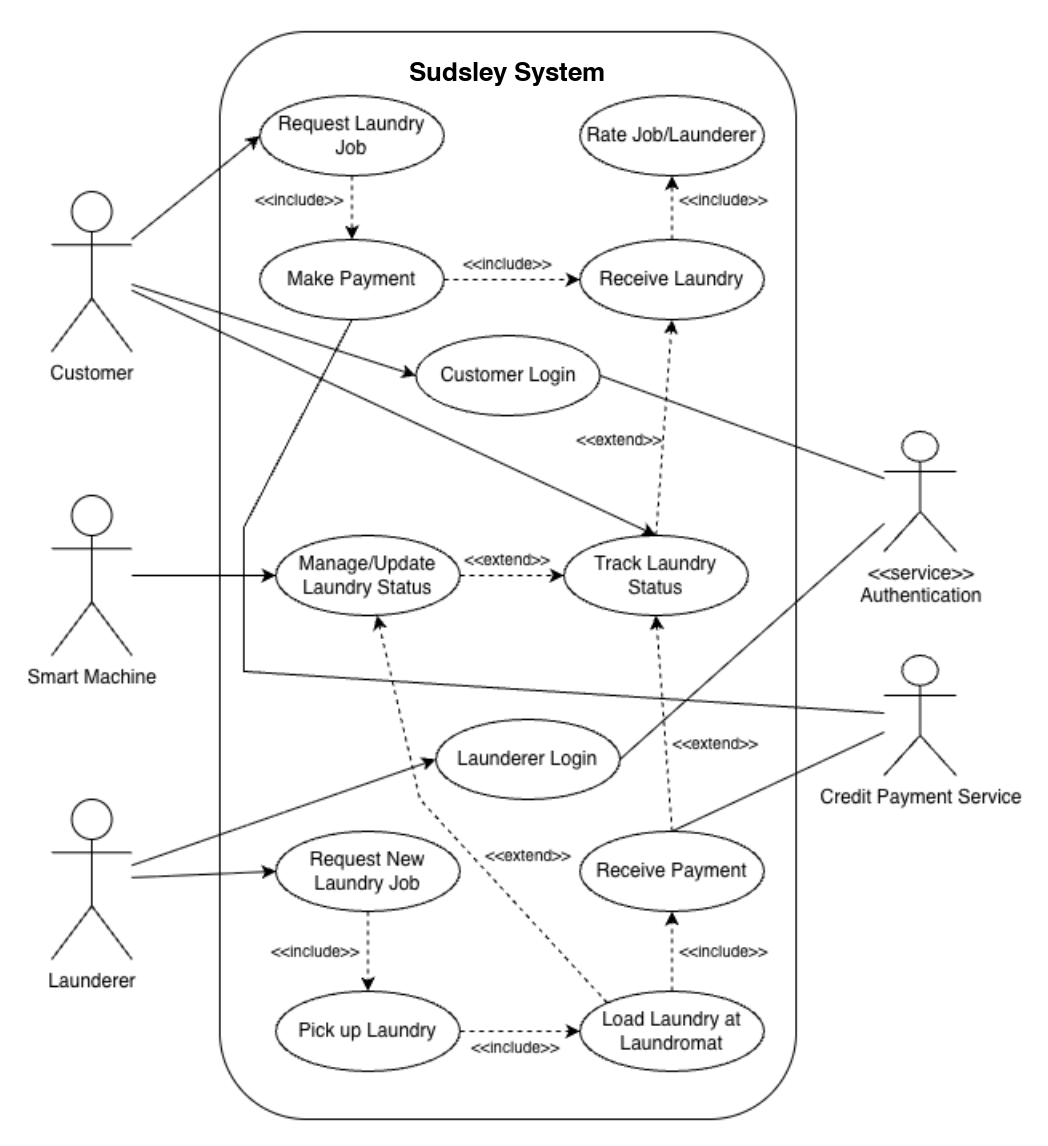
\includegraphics[height=0.82\textheight]{../assignments/hw1-high-level-design/example/use-case-diagram.png}
\end{frame}

\begin{frame}{Clients}
  There is a mobile app for each type of user.
  \begin{itemize}
    \item \textbf{Customer App} and \textbf{Launderer App}
    \item Distinct purposes, slightly different API calls
    \item The frontend team builds them
  \end{itemize}
\end{frame}

\begin{frame}{Backend services}
  \small
  \begin{itemize}
    \item<1-> \textbf{Job Service.} The ``brain'': orchestrates the whole laundry process,
      from job creation and launderer matching to tracking the job's status. Its main purpose
      is to call and notify other services, so it is often called an \alert{orchestrator}.
    \item<2-> \textbf{Payment Service.} Charges customers and pays launderers, through the
      Payment Provider.
    \item<3-> \textbf{Location Service.} Tracks launderers in real time; gets ETAs and routes
      from the Maps Provider.
    \item<4-> \textbf{Machine Service.} Finds available machines at Sudsley locations and
      remotely starts and monitors cycles through the Smart Machine API.
    \item<5-> \textbf{User Service.} Customer and launderer profile data, separate from
      authentication: saved addresses, preferences, aggregated ratings.
    \item<6-> \textbf{Notification Service.} Real-time push notifications to customers and
      launderers about job updates.
  \end{itemize}
\end{frame}

\begin{frame}{External services}
  \small
  \begin{itemize}
    \item<1-> \textbf{Payment Provider} (e.g., Square, Stripe). Processes payments and
      payouts securely. We store no financial information.
    \item<2-> \textbf{Maps Provider} (e.g., Google Maps). Mapping, geocoding, route planning.
    \item<3-> \textbf{Identity Provider} (e.g., Auth0, Okta, Cognito). Sign-up, login, and
      credentials. We store no passwords or credentials.
    \item<4-> \textbf{Smart Machine API.} Our own proprietary API for controlling the
      machines. ``External'' in the sense that we treat it as a black box that works.
  \end{itemize}
\end{frame}

\begin{frame}{Sudsley high-level design}
  \centering
  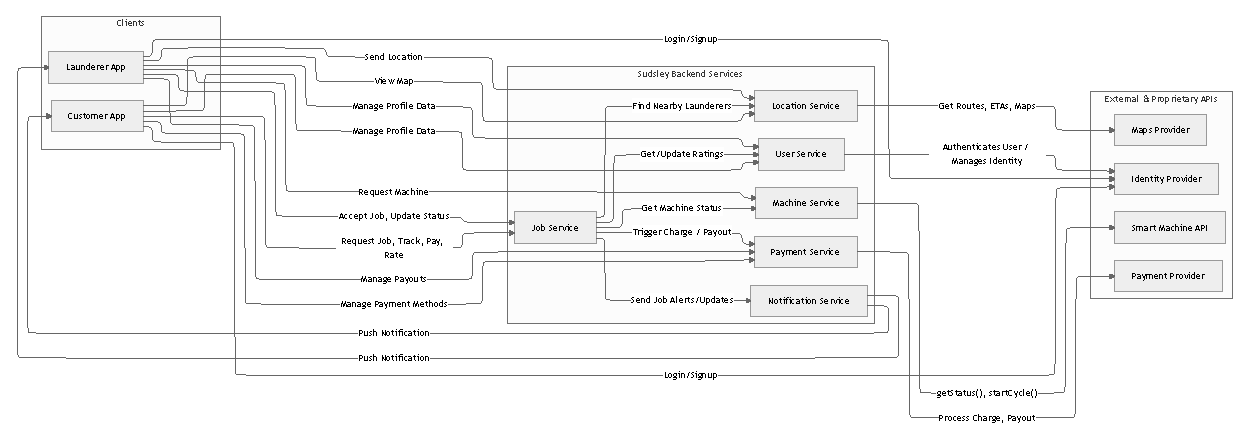
\includegraphics[width=\textwidth]{figures/high-level-design.pdf}
\end{frame}

\section{Component-level design}

\begin{frame}{From floor plan to schematic}
  \begin{itemize}
    \item \textbf{High-level design} is an architect's floor plan of a house: the kitchen,
      the bedrooms, the bathrooms.
    \item \textbf{Component-level design} is the schematic for just the kitchen: exactly
      where the sink, stove, and dishwasher go, and how their plumbing and wiring connect.
  \end{itemize}
\end{frame}

\begin{frame}{Define the component-level design}
  After the high-level (macro) design comes the component-level (micro) design.
  \begin{itemize}
    \item Zoom in on one component from the high-level diagram: a microservice, a client
      app, or an external API.
    \item Move from the \emph{what} (the components) to the \emph{how} (their implementation
      details).
  \end{itemize}
  A component-level design:
  \begin{itemize}
    \item defines specific responsibilities,
    \item describes the internal logic, and
    \item specifies interactions and dependencies: which services it calls and which
      external dependencies it relies on.
  \end{itemize}
\end{frame}

\begin{frame}{Component architecture questions}
  \begin{columns}[T]
    \begin{column}{0.5\textwidth}
      \small
      \begin{enumerate}
        \item What exact data fields should it store?
        \item Does it need an API? If so, what endpoints?
        \item What latency is acceptable?
        \item How consistent should it be?
        \item How much storage is needed?
        \item How many read vs.\ write requests?
        \item Is the data structured and relational, or more flexible?
      \end{enumerate}
    \end{column}
    \begin{column}{0.5\textwidth}
      \small
      \begin{enumerate}
        \setcounter{enumi}{7}
        \item How will the service scale?
        \item Does it need a cache?
        \item Is it stateless?
        \item Does it need rate limiting?
        \item What key metrics should it log?
        \item Does it have external dependencies? What are the limits?
      \end{enumerate}
    \end{column}
  \end{columns}
  \medskip
  \centering\alert{Let's design the User Service.}
\end{frame}

\begin{frame}{User Service: data, API, latency}
  \begin{qtable}
    \qrow{1. What data fields should it store?}
      {The data model: what this service owns, separate from data other services manage.}
      {Customer: \texttt{user\_id}, \texttt{display\_name}, \texttt{saved\_address},
       \texttt{laundry\_preferences}.\newline
       Launderer: \texttt{user\_id}, \texttt{display\_name}, \texttt{average\_rating},
       \texttt{total\_ratings}, \texttt{is\_active}.}
    \qrow{2. Does it need an API?}
      {The service's contract: what other services and the apps can call.}
      {Yes. \texttt{GET} and \texttt{POST /users/\{user\_id\}};
       \texttt{GET} and \texttt{POST /launderers/\{launderer\_id\}/rating}.}
    \qrow{3. What latency is acceptable?}
      {The speed target, which drives database and caching choices.}
      {Reads very fast: under 150\,ms at p99. Writes can be slower: under 500\,ms.}
  \end{qtable}
\end{frame}

\begin{frame}{User Service: consistency, storage, traffic}
  \begin{qtable}
    \qrow{4. How consistent should it be?}
      {Must a write be readable everywhere immediately (strong), or is a short delay fine
       (eventual)?}
      {Eventual. A profile update can take a few seconds to propagate; not every customer
       needs a new rating right away.}
    \qrow{5. How much storage is needed?}
      {A capacity estimate, to pick a database plan and prepare for scaling.}
      {Very little at first: 10k users $\times$ 5\,KB = 50\,MB, trivial for a modern
       database.}
    \qrow{6. How many reads vs.\ writes?}
      {The traffic pattern, which drives the database and caching strategy.}
      {Highly read-heavy, about 100:1. Profiles are read on every app open; ratings are read
       constantly and written once per job.}
  \end{qtable}
\end{frame}

\begin{frame}{Is eventual consistency always fine?}
  A customer changes \texttt{saved\_address}, then requests a pickup straight away.
  \pause
  \begin{itemize}
    \item The Job Service reads the profile before the update has propagated.
    \item The launderer goes to the old address.
  \end{itemize}
  \pause
  Fields the next request depends on need \alert{read-your-writes} consistency: read them
  from the primary database, not a replica or the cache, right after an update.
\end{frame}

\begin{frame}{User Service: database, scaling, cache}
  \begin{qtable}
    \qrow{7. Relational or flexible data?}
      {SQL for structured, relational data; NoSQL for flexible documents that scale more
       easily.}
      {NoSQL (e.g., DynamoDB, MongoDB). A profile is self-contained, one document suits a
       read-heavy load, and the schema can grow.}
    \qrow{8. How will the service scale?}
      {From 10k to 10M users: a bigger server (vertical) or more identical servers
       (horizontal).}
      {Horizontally: identical instances behind a load balancer. Possible because the
       service is stateless.}
    \qrow{9. Does it need a cache?}
      {A fast in-memory store (e.g., Redis) in front of the database for frequently read
       data.}
      {Yes. Read-heavy and rarely changing, so check the cache first and skip the database:
       faster responses, protected database.}
  \end{qtable}
\end{frame}

\begin{frame}{User Service: state, limits, metrics}
  \begin{qtable}
    \qrow{10. Is it stateless?}
      {Does it remember anything between requests, or get everything with each request?}
      {Completely stateless. Each request carries an Identity Provider token, so any server
       can handle any request.}
    \qrow{11. Does it need rate limiting?}
      {A security and cost control: cap requests per user or IP address.}
      {Yes, on writes, so a script can't change an address 1,000 times a second. For example,
       10 profile updates per minute.}
    \qrow{12. What key metrics should it log?}
      {You can't fix what you can't see.}
      {Request latency at p99, error rate, and cache hit rate.}
  \end{qtable}
\end{frame}

\begin{frame}{User Service: dependencies}
  \begin{qtable}
    \qrow{13. External dependencies? Limits?}
      {What it relies on, and what happens when each dependency fails.}
      {Three. If the \textbf{database} is down, nothing can be read or written. If the
       \textbf{cache} is down, reads fall back to the database: slower, but working. If the
       \textbf{Identity Provider} is down, tokens can't be validated and every request fails
       authentication.}
  \end{qtable}
\end{frame}

\begin{frame}{User Service component design}
  \centering
  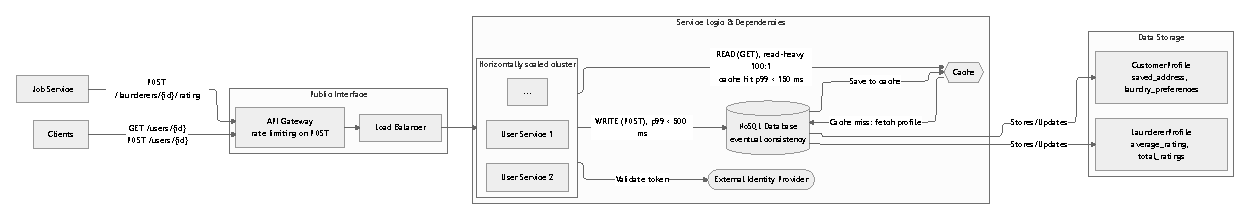
\includegraphics[width=\textwidth]{figures/user-service.pdf}
\end{frame}

\begin{frame}{Homework 2: component-level design (individual, collaboration permitted)}
  Draft a component-level design for the \alert{Machine Service}:
  \begin{enumerate}
    \item Review the finished high-level design.
    \item Answer the thirteen component architecture questions.
    \item Create a rough design diagram. Mermaid is a useful tool:
      \url{https://mermaid.js.org/}
  \end{enumerate}
  \handout{assignments/hw2-component-design/HOMEWORK.md}
\end{frame}

\end{document}
